\documentclass{article}
\usepackage{algorithm}
\usepackage{algpseudocode}
\usepackage{amsmath,amssymb,amsthm}
\usepackage{graphicx}
\usepackage[margin=1in]{geometry}
\usepackage{fancyhdr}
\usepackage{float}
\usepackage{longtable}
\setlength{\parindent}{0pt}
\setlength{\parskip}{5pt plus 1pt}
\setlength{\headheight}{13.6pt}
\newcommand\question[2]{\vspace{.25in}\hrule\textbf{#1: #2}\hrule\vspace{.10in}}
\renewcommand\part[1]{\vspace{.10in}\textbf{(#1)}}
\newcommand\algo{\vspace{.10in}\textbf{Algorithm: }}
\newcommand\correctness{\vspace{.10in}\textbf{Correctness: }}
\newcommand\runtime{\vspace{.10in}\textbf{Running time: }}
\newcommand\pseudoCode{\vspace{.10in}\textbf{PseudoCode: }}
\newcommand*{\perm}[2]{{}^{#1}\!P_{#2}}
\newcommand*{\comb}[2]{{}^{#1}\!C_{#2}}
%\pagestyle{fancyplain}
%\lhead{\textbf{\NAME\ (\UID)}}
%\chead{\textbf{Hw\HWNUM}}
%\rhead{CS 6350, \today}
\title{CS6350 - Homework/Assignment-5}
\author{Arnab Das(u1014840)}
\usepackage[utf8]{inputenc}
\begin{document}
  \pagenumbering{gobble}
  \maketitle
  \newpage
  \pagenumbering{arabic}
  \newcommand\NAME{ARNAB DAS}
  \newcommand\UID{uxxxxxxx}
  \newcommand\HWNUM{4}

  \question{1}{Margins}
  \part{1} For a xor function in two dimension of $x_{1},x_{2}$ and label $y$, the examples sets in the form of tuple $(x_1, x_2, y)$ are $(-1,-1,-1)$, $(-1,1,1)$, $(1,-1,1)$ and $(1,1,-1)$, where variables are boolean and takes $\{-1,1\}$. It is not linearly separable in the euclidean space. However, the transformation, $\phi$, of mapping $[x_1, x_2]$ to $[x_1, x_1x_2]$ makes it linearly separable in which the datapoints now $(x_1, x_1x_2, y)$ becomes $(-1,1,-1)$, $(-1,-1,1)$, $(1,-1,1)$ and $(1,1,-1)$. The line $x_1x_2=0$ is a separating classifier. SInce $x_1x_2=0$ is equaidistant from all the 4 points in the transformed space, it gives the maximum margin, which is the distance of any of the points(since equidistant) from this line. and equal to \textbf {1 unit}.  The linear classifier in the transformed space when mapped back to the original euclidean space , will be combination of the lines $x_1=0$ and $x_2=0$, as shown in Figure-1(c). This is because in the transformed space, since $x_1x_2=0$ means that line satisfies all points which has $x_1=0$ or/and $x_2=0$, hence in the euclidean space it is a combination of both. \newline

  \begin{figure}[H]
   \centering
  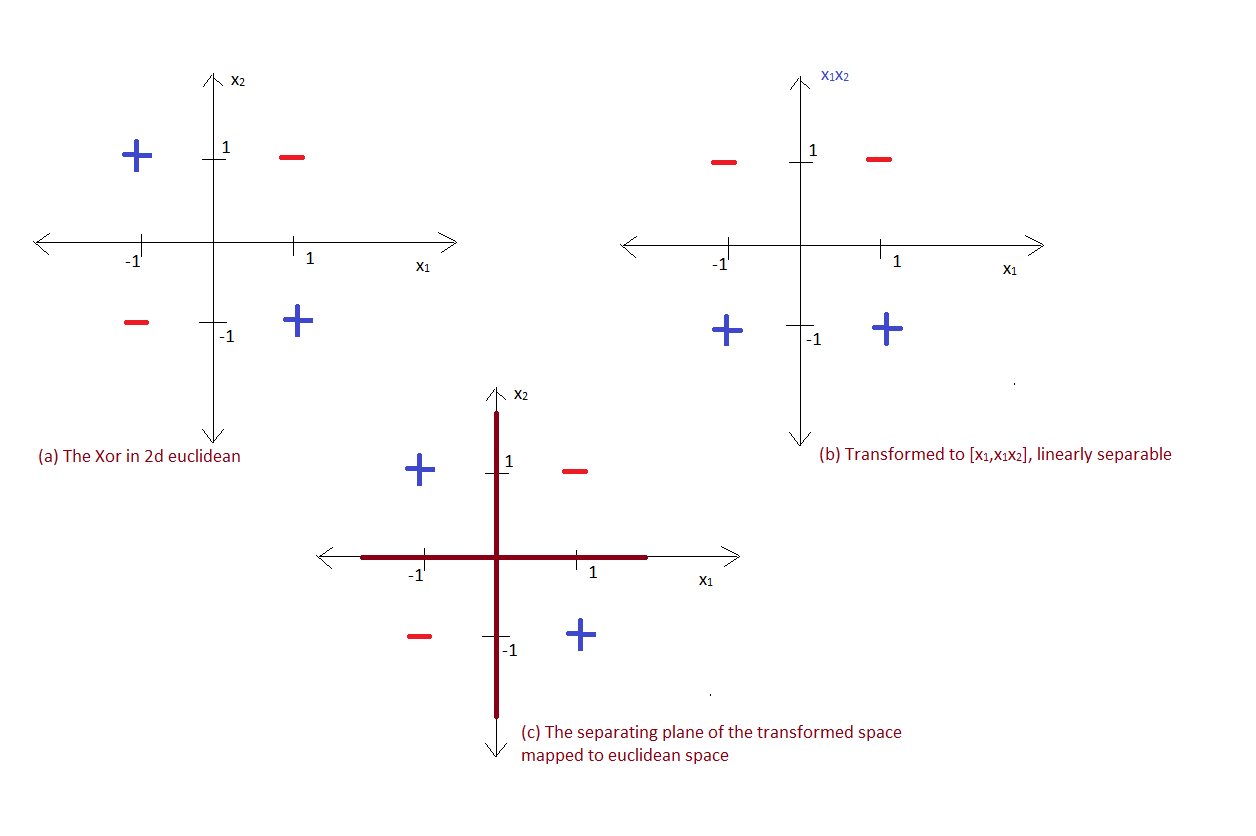
\includegraphics[width=12cm, height=12cm]{Prob1a}
  \caption{Space transformation for Xor to make linearly separable}
  \end{figure}

  \part{2a} For $D_1 = \{x_1, x_2, x_3, x_5, x_7\}$, the linear classifier with the maximum margin will be parallel to the line joining $x_1$ and $x_3$, and the distance of this classifer will be equal from $x_1 and x_3$ on one side and $x_5$ on the other side.  Hence, the maximum possible margin for $D_1$ will be half the distance of $x_5$ from the line joining $x_1$ and $x_3$. The line joining $x_1,x_3$ is $x_1 - x_2 = 0$. Then, margin for $D_1$ will be: \newline
  \[D_{1_{marginMax}} = \dfrac{1}{2 \times \sqrt[2]{2}}\]
 
    For $D_2 = \{ x_1, x_5, x_6, x_8\}$, the linear classifier with the maximum margin will be parallel to the line joining $x_5, x_6$, and the distance of this classifier will be equal from $x_5$ and $x_6$ on one side and $x_1$ on the other side. Hence, the maximum possible margin for $D_2$ will be half of the distance of $x_1$ from the line joining $x_5$ and $x_6$. The line joining $x_5, x_6$ is $\sqrt[2]{3}x_1 + x_2 - \sqrt[2]{3} = 0$. Then the margin for $D_2$ will be: \newline
    \[D_{2_{marginMax}} = \dfrac{\sqrt[2]{3}}{4} \]

    For $D_3 = \{ x_3, x_4, x_5, x_7 \}$, the linear classifier with the maximum margin will be parallel to the line joining $x_4$ and $x_3$, and the distance of this classifier will be equal from $x_4$ and $x_3$ from one side and from $x_5$ on the other side. Hence, the maximum possible margin for $D_3$ will be half of the distance of $x_5$ from the line joining $x_3$ and $x_4$. The line joining $x_3$ and $x_4$ is $2x_1 - x_2 - 1 = 0$. Then the margin for $D_3$ will be: \newline
    \[ D_{3_{marginMax}} = \dfrac{1}{2\times \sqrt[2]{5}}\]

    \part{2b}
    For $D_1$, $R=\dfrac{3}{2}$ and $\gamma = \dfrac{1}{2 \times \sqrt[2]{2}}$, perceptron mistake bound for $D_1$ = 18. \newline
    For $D_2$, $R=1$ and $\gamma=\dfrac{\sqrt[2]{3}}{4}$, perceptron mistake bound for $D_2$ = $\dfrac{16}{3}$. \newline
    For $D_3$, $R=\dfrac{3}{2}$ and $\gamma = \dfrac{1}{2\times \sqrt[2]{5}}$, perceptron mistake bound for $D_3$ = 45. \newline
    $D_3$ has the greatest mistake bound. \newline

    \part{2c} A higher mistake bound indicates how well the classifier can fit the training data by making only this bounded number of mistakes. Hence, a low mistake bound will means the classifier fits the training data quickly. However, that provides no guarantees on the test data. Since the perceptron learns by making mistakes, hence a lower number of mistakes indicate that the learning performed by the perceptron has been less, and hence its predictive power intuitively reduces on the test data. To put it simply, a classifier learns less if it makes less number of mistakes because that is its only entry point towards learning and updates. Hence, the classifier with a higher mistakes bound is easier to learn and the one with a small mistake bound is difficult to learn. Thus the ranking in order of ease of ranking will be $D_3$, $D_1$, $D_2$ . \newline
\end{document}
